%versi 2 (8-10-2016)
\chapter{Landasan Teori}
\label{chap:teori}

Pada bab ini akan diuraikan teori-teori yang akan digunakan untuk pembangunan aplikasi ke analisis kota Bandung. Teori-teori tersebut adalah tentang protokol HTTP, \textit{library} Jsoup meliputi kelas jsoup dan Connection. Selain itu akan dibahas juga mengenai \textit{JavaScript Object Notation (JSON)} meliputi kelas pada \textit{library} JSON : JSONObject dan \textit{Google Direction API}.

\section{Protokol HTTP}
\label{sec:protocolhttp} 

HTTP(\textit{HyperText Transfer Protocol}) adalah protokol di balik World Wide Web. Dengan setiap transaksi web, HTTP dipanggil. HTTP adalah di balik setiap permintaan dokumen web atau grafis, setiap klik link hypertext, dan setiap penyerahan formulir. Web adalah tentang penyebaran informasi melalui Internet, dan HTTP adalah protokol yang digunakan untuk melakukannya.

\subsection{Transaksi HTTP}
\label{subsec:architecturehttp}

Berikut akan diilustrasikan transaksi web umum, menunjukkan HTTP yang dipertukarkan antara program \textit{client} dan \textit{program} server. \cite{wong2000http}:

\begin{itemize}
	\item berikut diberikan sebuah url : http://hypothetical.ora.com:80/.
	\item Browser akan mengintepretasikan URL tersebut sebagai berikut :
			\begin{itemize}
				\item \(http://\) : menggunakan protokol HTTP.
				\item \(hypothetical.ora.com\) : menghubungi komputer melalui jaringan dengan hostname hypothetical.ora.com.
				\item \(:80\) : Terhubung ke komputer di port 80. Nomor port IP nomor dari 1 sampai 65535. Jika titik dua dan nomor port dihilangkan, nomor port diasumsikan nomor port \textit{default} HTTP, yang merupakan 80.
				\item \(\/\) : Apapun setelah nama host dan nomor port opsional dianggap sebagai jalan dokumen. Dalam ilustrasi ini, jalan dokumen adalah \/.
			\end{itemize}
			\item Pada ilustrasi ini browser menghubungkan ke hypothetical.ora.com pada port 80 menggunakan protokol HTTP. Pesan bahwa browser mengirimkan ke server adalah sebagai berikut:
			\begin{figure}[H]
				\centering		
				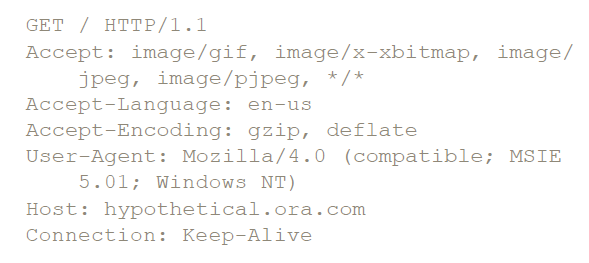
\includegraphics[scale=0.7]{Gambar/request.png}
				\caption[HTTP Request]{HTTP Request\cite{wong2000http}}
				\label{fig:httprequest}	
			\end{figure}
\end{itemize}
\begin{itemize}
	\item Pada baris pertama pada request (Gambar \ref{fig:httprequest}) disebut dengan request line dan diawali dengan \textit{request method}(metode permintaan), dalam gambar tersebut adalah GET. \textit{Request method} diikuti dengan \textit{resource} yang diinginkan, dalam gambar tersebut adalah /. \textit{Request line} diakhiri dengan versi protokol yang digunakan dalam gambar diatas adalah HTTP/1.1.
	\item baris kedua dan baris-baris berikutnya sampai ditemukan baris kosong, berisi request headers dalam format \textit{nama-header:nilai-header}. pada gambar \ref{fig:httprequest} terdapat header host yang menandakan bahwa browser ingin mengakses situs dari nilai yang ada di header host.
	\item Dibawah header-header pada gambar \ref{fig:httprequest} terdapat baris kosong di akhir \textit{request}. pada \textit{request}, baris kosong memisahkan antara \textit{request headers} dengan \textit{request body}(tubuh permintaan).
\end{itemize}

Setelah \textit{client} memberikan \textit{request} server memberikan \textit{response}. Dari kasus diatas berikut adalah sebagai berikut :
			\begin{figure}[H]
				\centering		
				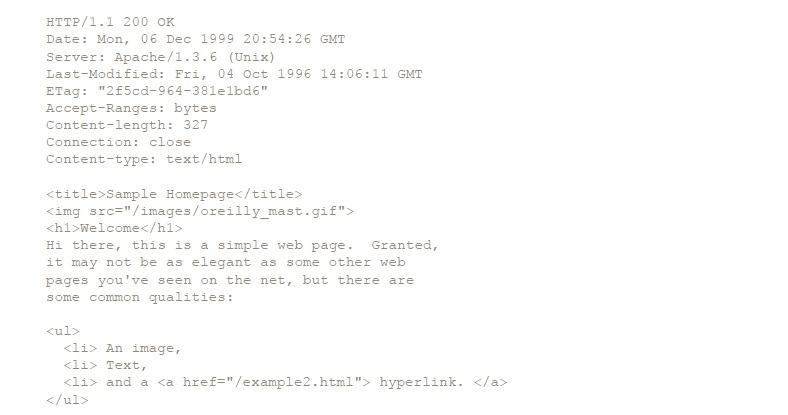
\includegraphics[scale=0.6]{Gambar/respondserver.jpg}
				\caption[HTTP Respond]{HTTP Respond\cite{wong2000http}}
				\label{fig:httprespond}	
			\end{figure}
 \begin{itemize}
	\item Pada baris pertama pada respon (Gambar \ref{fig:httprespond}) disebut \textit{status line}, dan diawali dengan versi protokol yang digunakan, dalam kasus ini HTTP/1.1. \textit{Status line} diikuti dengan 3 dijit kode status, dalam kasus ini 200. \textit{Status line} diakhiri dengan representasi tekstual dari status tersebut dalam kasus ini \textit{OK}.
	\item Baris kedua dan baris-baris berikutnya sampai ditemukan baris kosong, berisi request headers dalam format \textit{nama-header:nilai-header}. pada gambar \ref{fig:httprespond} terdapat header server yang menandakan bahwa server yang digunakan untuk melayani request.
	\item Setelah baris kosong adaah \textit{body} dari \textit{response}, gambar \ref{fig:httprespond} berupa teks HTML.
	\item Pada gambar \ref{fig:httprespond} ada kebutuhan akan \textit{file} oreilly\_mast.gif di HTML ini. \textit{File} tersebut akan diunduh secara terpisah, tetapi juga dengan protokol HTTP.
\end{itemize}

Setelah semua terjadi dan dibaca dengan baik, maka baris kosong dan teks dokumen muncul. dengan demikian transaksi yang terjadi adalah sebagai berikut : 

			\begin{figure}[H]
				\centering		
				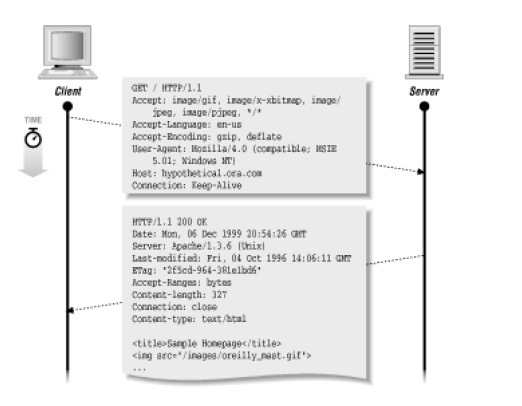
\includegraphics[scale=0.6]{Gambar/transaction.jpg}
				\caption[Transaksi sederhana]{Transaksi Sederhana\cite{wong2000http}}
				\label{fig:transaction}	
			\end{figure}
Berdasarkan gambar \ref{fig:transaction} terjadi transaksi data antara \textit{client} dan \textit{server} berikut adalah penjelasannya.
\begin{enumerate}
	\item \textit{Client} melakukan \textit{request} dengan \textit{header} \textit{get}. Selain itu juga terdapat \textit{header hostname hypotetical.ora.com} yang menjelaskan hostname yang dituju. Pada \textit{request} tersebut terdapat header protokol HTTP dan juga versi berapa yang digunakan. 
	\item Diterima oleh \textit{server} dan \textit{server} kemudian membalas dengan \textit{header} ok. Arti \textit{header} tersebut adalah \textit{request} yang diterima telah tersampaikan dengan baik dan mengembalikan HTML yang diminta ke \textit{client}. Dari \textit{respond} tersebut terdapat header : tanggal detail meliputi waktu pada saat melakukan \textit{respond}, protokol HTTP dan versi yang digunakan. Selain itu \textit{respond} ini juga mengandung \textit{body} dari HTML yang diminta.   
\end{enumerate}

\subsection{Kode Status}
\label{subsec:kodestatus}

Kode status adalah bilangan bulat tiga dijit yang menyatakan status dari pemrosesan permintaan yang dikirimkan. Berikut adalah beberapa kode status yang umum ditemui : 

\begin{table}[H]
\centering
\begin{tabular}{|p{3cm}|p{5cm}|p{5cm}|}
\hline
\textbf{Kode Status} & \textbf{Status}               & \textbf{Deskripsi}\\\hline
200         & OK                   & Request berhasil diproses dengan baik.                                                                                                                                         \\\hline
301         & Moved Permanently    & Resource yang diminta sudah berpindah ke URI yang lain secara permanen.                                                                                                        \\\hline
302         & Found                & Resource yang diminta untuk sementara bepindah pada URL yang lain. Untuk alasan historis, client diperkenankan untuk mengubah metode permintaan dan POST menjadi GET.          \\
307         & Temporary Redirect   & Resource yang diminta untuk sementara berpindah pada URL yang lain. Mirip dengan status 302 namun client tidak diperkenankan mengubah metode permintaan dari POST menjadi GET. \\\hline
400         & Bad Request          & Server tidak dapat memproses permintaan karena ada kesalahan adri client                                                                                                       \\\hline
401         & Unauthorized         & Server tidak dapat memproses permintaan karena kredensial diperlukan dan client tidak menyediakannya.                                                                          \\\hline
404         & Not Found            & Resource yang diminta tidak tersedia pada server.                                                                                                                              \\\hline
500         & Internal Server Error & Server mengalami masalah internal, sehingga tidak dapat memproses permintaan yang dikirimkan.                                                                                  \\\hline
501         & Not Implemented      & Server belum atau tidak mendukung fungsionalitas yang diminta oleh client.                                                                                                     \\\hline
503         & Service Unavailable  & Server tidak dapat menjawab permintaan client, karena terlalu sibuk atau perawatan. Status ini mengindikasikan client dapat mencoba lagi setelah jangka waktu tertentu.  \\\hline     
\end{tabular}
\caption[Tabel Kode Status]{Tabel Kode Status}
\label{table:kodestatus}
\end{table}

kode status yang tersedia dikelompokan menjadi lima, diindikasikan oleh dijit pertama dari kode tersebut:
\begin{itemize}
	\item 1xx(informational): Request diterima, dan proses dilanjutkan.
	\item 2xx(Successfull): Request diterima, dan dimengertian dengan baik.
	\item 3xx(Redirection): Aksi tambahan diperlukan untuk menyelesaikan permintaan.
	\item 4xx(Client Error): Terjadi kesalahan dan client harus memperbaikinya
	\item 5xx(Server Error):  Terjadi kesalahan pada sisi server.
\end{itemize}

\subsection{\textit{Request method}}
\label{subsec:requestmethod}

\textit{Request method} menentukan karakteristik dari permintaan yang dikirimkan. Ada 2 \textit{method} yang sudah dikenal umum yaitu GET dan POST. Selain kedua method tersebut, ada beberapa \textit{method-method} lain yang dapat juga digunakan pada protokol HTTP seperti dijelaskan pada tabel berikut: 

\begin{table}[H]
\centering
\begin{tabular}{|p{3cm}|p{6cm}|}
\hline
\textbf{Metode} & \textbf{Deskripsi}                                                                                                                                                                        \\\hline
GET    & Metode yang paling umum digunakan, dan digunakan untuk mendapatkan konten dari resource yang ditentukan pada request.                                                            \\\hline
POST   & Metode ini digunakan untuk meminta server memproses data yang dikirimkan. Pada umumnya, metode POST diikuti dengan request body, yang berisi parameter-parameter yang dikirimkan \\\hline
HEAD   & Metode HEAD mirip dengan metode GET, tetapi bedanya di sini server tidak mengembalikan konten body, melaikan hanya sampai response headers saja.                                 \\\hline
PUT    & Metode ini digunakan untuk membuat atau menggantikan resource yang ditentukan pada request.                                                                                      \\\hline
DELETE & Metode ini digunakan untuk menghapus resource dari server.             \\\hline                                                                                                       
\end{tabular}
\caption[Tabel Request Method]{Tabel Request Method}
\label{table:requestmethod}
\end{table}



\subsection{\textit{Response Headers}}
\label{subsec:responseheaders}

\textit{Response Headers} digunakan untuk meberikan informasi-informasi tambahan pada sebuah jawaban. Sama seperti \textit{request header}, setiap header terdiri dari nama dan nilai, dan terpisah oleh titik dua dan spasi(: ). Tabel berikut menjelaskan beberapa header yang umum dipakai:


\begin{table}[H]
\centering
\begin{tabular}{|p{3cm}|p{6cm}|}
\hline
\textbf{Header}        & \textbf{Deskripsi}                                                                                                                                                                                                                                                                                                                                                                                                                                                   \\\hline
Content-Type  & Header ini menunjukan tipe media dari konten yang akan diberikan. Pada bentuk sederhana, nilai dari header ini berisi dari kode tipe MIME(Multipurpose Internet Mail Extension). Beberapa kode tipe MIME yang umum antara lain: text/plain untuk teks, text/html untuk halaman HTML; image/gif, image/jpg, image/png untuk gambar berformat GIF, JPEG, PNG; dan application/json untuk data JSON.                                                           \\\hline
Cache-control & Header ini mengatur bagaimana konten yang dikirimkan dapat dikirimkan sementara di client. Pada konten-konten statis seperti gambar, secara default konten akan disimpan pada client dalam jangka waktu tertentu, sehingga jika dibutuhkan dalam waktu dekat di masa depan, tidak perlu mengirimkan permintaan lagi ke server. jika secara eksplisit diinginkan konten diminta lagi setiap kali diperlukan, dapat mengisi header ini dengan nilai no-cache. \\\hline
Location      & Header ini digunakan untuk beberapa jenis jawaban untuk menunjukan lokasi sumberdaya dalam bentuk URI. Pada jawaban dengan kode 3xx, nilai dari header ini menunjukan lokasi baru yang harus dituju.               \\\hline                                                                                                                        
\end{tabular}
\caption[Tabel Response Headers]{Tabel Response Headers}
\label{table:responseheaders}
\end{table}

\section{\textit{Library} jsoup}
\label{sec:libraryjsoup}

Jsoup adalah sebuah \textit{library} java untuk bekerja dengan HTML dunia nyata.  Jsoup menyediakan API yang sangat nyaman untuk mengekstrak dan memanipulasi data, menggunakan DOM(\textit{Document Object Model}), CSS(\textit{Cascading Style Sheets}), dan \textit{method} yang mirip dengan jquery. Jsoup mengimplementasikan spesifikasi standar \textit{WHATWG(\textit{Web Hypertext Application Technology Working Group}) HTML5} dan mengurai HTML menjadi DOM(Document Object Model) yang sama dengan peramban modern lakukan. Jsoup sendiri dirancang untuk menangani semua jenis HTML yang biasa ditemukan dengan membuat \textit{parsing tree} yang dapat dimengerti.

Dalam subbab berikut akan dijelaskan fungsi dan beberapa kelas dari jsoup\cite{jonathanhedley2016}.
\subsection{Fungsi jsoup}
\label{subsec:fungsijsoup}
berikut adalah fungsi dari jsoup :

\begin{itemize}
	\item menghimpun dan mengurai HTML dari URL, file, atau \textsl{string}.
	\item mencari dan mengambil data, menggunakan \textit{DOM traversal} atau \textit{CSS selectors}.
	\item memanipulasi elemen HTML, atribut, dan teks.
	\item membersihkan konten yang dikirimkan pengguna terhadap daftar putih yang aman, untuk mencegah serangan XSS.
	\item memberi \textit{output} HTML yang rapi.
\end{itemize}

\subsection{Kelas- kelas jsoup}
\label{subsec:jsoupclasses}

\subsubsection{Jsoup}
\label{subsubsec:jsoup}
Kelas ini merupakan inti untuk mengakses fungsi jsoup. Seluruh method dalam kelas ini merupakan \textit{static method} sehingga kelas ini tidak perlu dikonstruksi. Salah satu method yang dimiliki kelas ini adalah sebagai berikut :
\begin{itemize}
	\item \textbf{public static Connection connect(String url)}
	
	Berfungsi untuk membuat koneksi baru dengan suatu situs web.
	
	Parameter:
	\begin{itemize}
		\item \textbf{url}: URL situs web dengan protokol HTTP.
	\end{itemize}
	\textbf{Kembalian}: koneksi dengan situs web.
\end{itemize}

\subsubsection{Connection}
\label{subsubsec:connection}

Kelas ini merupakan interface yang menyediakan pengambilan data dari situs web. Beberapa method yang dimiliki kelas ini adalah sebagai berikut:
\begin{itemize}
	\item \textbf{Connection data(String key, String value)}
	
	Berfungsi untuk menambahkan parameter data yang bisa dikirim melalui metode HTTP GET atau POST.
	
	Parameter:
	\begin{itemize}
		\item \textbf{key}: kunci data.
		\item \textbf{value}: nilai data.
	\end{itemize}
	\textbf{Kembalian}: koneksi yang sama tetapi sudah diubah.
	
	\item \textbf{Connection ignoreContentType(boolean ignoreContentType)}
	
	Berfungsi untuk Mengabaikan tipe konten dokumen saat \textit{parsing} respon.
	
	Parameter:
	\begin{itemize}
		\item \textbf{ignoreContentType}: set true jika ingin jenis konten diabaikan pada \textit{parsing} respon dalam dokumen.
	\end{itemize}
	\textbf{Kembalian}: koneksi pada situs web.
	
	\item \textbf{Connection.Response execute() throws IOException}
	
	Berfungsi untuk mengeksekusi \textbf{request} dari \textbf{Connection}.
	
	\textbf{Kembalian}: objek respon.
	
	\item \textbf{String body()}
	
	Berfungsi untuk mendapatkan \textit{body} respon sebagai string biasa.
	
	\textbf{Kembalian}: \textit{string} dari \textit{body}.
\end{itemize}

\section{\textit{JavaScript Object Notation (JSON)}}
\label{sec:json}
JSON (JavaScript Object Notation) adalah format pertukaran data yang ringan, mudah dibaca dan ditulis oleh manusia, serta mudah diterjemahkan dan dibuat (generate) oleh komputer. Format ini dibuat berdasarkan bagian dari Bahasa Pemprograman JavaScript, Standar ECMA-262 Edisi ke-3 - Desember 1999. JSON merupakan format teks yang tidak bergantung pada bahasa pemprograman apapun karena menggunakan gaya bahasa yang umum digunakan oleh programmer keluarga C termasuk C, C++, C\#, Java, JavaScript, Perl, Python dll\cite{ecmainternational2013}.

\subsection{Struktur JSON}
\label{subsec:stukturjson}
JSON terbuat dari dua struktur :
\begin{itemize}
	\item Kumpulan pasangan nama/nilai.
	\item Daftar nilai terurutkan (an ordered list of values).
\end{itemize} 

Struktur-struktur data ini disebut sebagai struktur data universal. Pada dasarnya, semua bahasa pemprograman moderen mendukung struktur data ini dalam bentuk yang sama maupun berlainan. Hal ini pantas disebut demikian karena format data mudah dipertukarkan dengan bahasa-bahasa pemprograman yang juga berdasarkan pada struktur data ini.

\subsection{Bentuk-Bentuk JSON}
\label{subsec:bentukjson}
\begin{itemize}
	\item Objek
	
	Objek adalah sepasang nama/nilai yang tidak terurutkan. Objek dimulai dengan { (kurung kurawal buka) dan diakhiri dengan } (kurung kurawal tutup). Setiap nama diikuti dengan : (titik dua) dan setiap pasangan nama atau nilai dipisahkan oleh , (koma).
	\begin{figure}[H]
		\centering		
		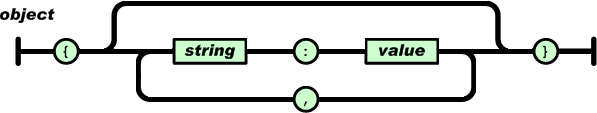
\includegraphics[scale=0.4]{Gambar/object.png}
		\caption[JSON Object]{JSON Object}
		\label{fig:jsonobject}	
	\end{figure}
	\item \textit{Array}
	
	\textit{Array} adalah kumpulan nilai yang terurutkan. Larik dimulai dengan [ (kurung kotak buka) dan diakhiri dengan ] (kurung kotak tutup). Setiap nilai dipisahkan oleh , (koma).
	\begin{figure}[H]
		\centering		
		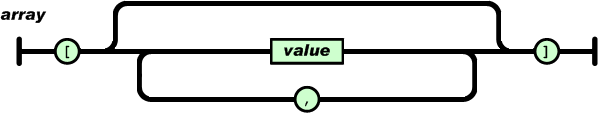
\includegraphics[scale=0.4]{Gambar/array.png}
		\caption[JSON Object]{JSON Array}
		\label{fig:jsonarray}	
	\end{figure}
\end{itemize} 

\subsection{Value JSON}
\label{subsec:valuejson}

Nilai(\textit{value})dapat berupa sebuah string dalam tanda kutip ganda, atau angka, atau true atau false atau null, atau sebuah objek atau sebuah larik. Struktur-struktur tersebut dapat disusun bertingkat.
\begin{figure}[H]
	\centering		
	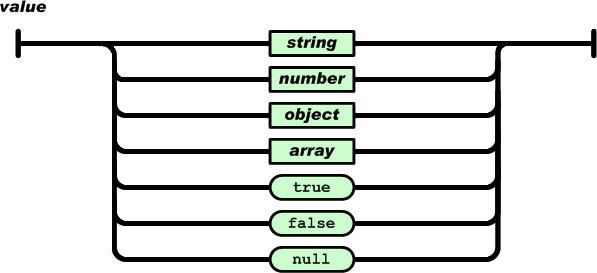
\includegraphics[scale=0.4]{Gambar/value.png}
	\caption[Value]{Value}
	\label{fig:value}	
\end{figure}

\begin{itemize}
\item{\textit{String}}

String adalah kumpulan dari nol atau lebih karakter Unicode, yang dibungkus dengan tanda kutip ganda. Di dalam string dapat digunakan backslash escapes "\" untuk membentuk karakter khusus. Sebuah karakter mewakili karakter tunggal pada string. String sangat mirip dengan string C atau Java.

\begin{figure}[H]
	\centering		
	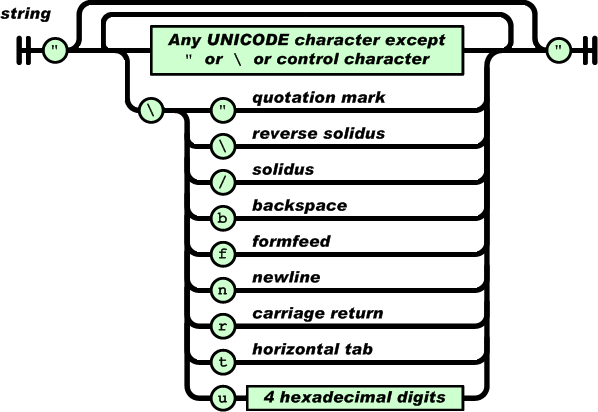
\includegraphics[scale=0.4]{Gambar/string.png}
	\caption[String]{String}
	\label{fig:string}	
\end{figure}

\item{Angka}

Angka adalah sangat mirip dengan angka di C atau Java, kecuali format oktal dan heksadesimal tidak digunakan.
\begin{figure}[H]
	\centering		
	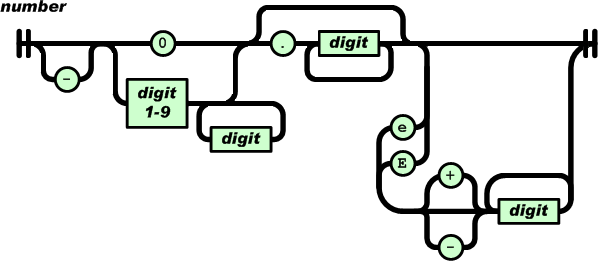
\includegraphics[scale=0.4]{Gambar/number.png}
	\caption[Angka]{Angka}
	\label{fig:number}	
\end{figure}
\end{itemize}

\subsection{kelas-kelas pada \textit{Library} JSON}
\label{subsec:jsonclasses}
Subbab-subbab berikut menjelaskan beberapa kelas dari \textit{library} JSON\footnote{https://stleary.github.io/JSON-java/}.

\subsubsection{JSONObject}
\label{subsubsec:jsonobject}
Kelas ini merepresentasikan sebuah objek JSON yang merupakan koleksi yang tak terurut dari pasangan nama dan nilai. Bentuk eksternal objek JSON adalah sebuah string dibungkus dalam kurung kurawal dengan titik dua antara nama dan nilai-nilai, dan koma antara nilai-nilai dan nama. Nilai-nilai dapat salah satu dari jenis: Boolean, JSONArray, JSONObject, Nomor, String, atau benda JSONObject.NULL. beberapa \textit{method} dan \textit{constructor} yang dimiliki kelas ini adalah sebagai berikut:

\begin{itemize}
	
	\item \textbf{public JSONObject(String source) throws JSONException}
	
	Berfungsi untuk membangun JSONObject dari sumber JSON string teks.
	
	Parameter:
	\begin{itemize}
		\item \textbf{source}: Sebuah string dimulai dengan \{(kurung kurawal kiri) dan berakhir dengan\} (kurung kurawal kanan).
	\end{itemize}
	
	\item \textbf{public String getString(String key)throws JSONException}
	
	Berfungsi untuk mendapatkan objek nilai yang terkait dengan kunci.
	
	Parameter:
	\begin{itemize}
		\item \textbf{key}: kunci data.
	\end{itemize}
	\textbf{Kembalian}: Sebuah string yang merupakan nilai.
	
	\item \textbf{public String optString(String key)}
	
	Berfungsi untuk mendapatkan string opsional terkait dengan kunci. Ia mengembalikan string kosong jika tidak ada kunci yang ditemukan. Jika nilai tidak string dan tidak null, maka dikonversi ke string.
	
	Parameter:
	\begin{itemize}
		\item \textbf{key}: kunci data.
	\end{itemize}
	\textbf{Kembalian}: Sebuah string yang merupakan nilai.
	
	\item \textbf{public JSONArray getJSONArray(String key) throws JSONException}
	
	Berfungsi untuk mendapatkan nilai JSONArray terkait dengan kunci.
	
	Parameter:
	\begin{itemize}
		\item \textbf{key}: kunci data.
	\end{itemize}
	\textbf{Kembalian}: Sebuah JSONArray yang merupakan nilai.
	
	\item \textbf{public JSONObject getJSONObject(String key) throws JSONException}
	
	Berfungsi untuk mendapatkan nilai JSONObject terkait dengan kunci.
	
	Parameter:
	\begin{itemize}
		\item \textbf{key}: kunci data.
	\end{itemize}
	\textbf{Kembalian}: Sebuah JSONObject yang merupakan nilai.
\end{itemize}

\section{Google Direction}
\label{sec:googledirapi}

Google Maps Directions adalah layanan yang menghitung arah antar lokasi menggunakan permintaan HTTP\cite{ankurkotwal2017}. Anda bisa mencari arah untuk beberapa moda transportasi, termasuk angkutan umum, mengemudi, berjalan atau bersepeda. Arah bisa menetapkan tempat asal, tujuan dan \textit{waypoint} baik sebagai string teks atau sebagai koordinat garis lintang/garis bujur. Layanan ini didesain untuk menghitung arah alamat statis (sudah diketahui sebelumnya) untuk penempatan konten aplikasi pada peta.

\subsection{Permintaan Arah}
\label{subsec:permintaanarahgoogledir}

Permintaan Google Maps Directions mengambil bentuk berikut:

\begin{lstlisting}[caption= \textit{Request} Google Directions\cite{ankurkotwal2017}, captionpos=b]
https://maps.googleapis.com/maps/api/directions/json?parameters
\end{lstlisting}

HTTP disarankan untuk aplikasi yang berisi data pengguna sensitif, seperti lokasi pengguna, dalam permintaan. URL Google Maps Directions API dibatasi sekitar 2000 karakter, setelah Pengkodean URL. Karena sebagian URL Google Maps Directions API bisa melibatkan banyak lokasi sepanjang lintasan. Pada subbab berikutnya akan dijelaskan parameter apa saja yang digunakan pada permintaan ke layanan ini.

\subsection{Parameter Permintaan}
\label{subsec:parameterpermintaangoogledir}

Beberapa parameter tertentu diperlukan sementara yang lainnya bersifat opsional. Sebagaimana standar dalam URL, semua parameter dipisah menggunakan karakter ampersand (\&). Daftar parameter dan kemungkinan nilainya disebutkan di bawah ini\cite{ankurkotwal2017}.

\subsubsection{Parameter yang diperlukan}
\label{subsubsec:parameterwajib}
\begin{itemize}
	\item \textbf{origin} adalah alamat, nilai garis lintang/garis bujur tekstual, atau ID tempat asal yang ingin Anda hitung arahnya. ketentuan dari alamat dari origin adalah sebagai berikut :
	\begin{itemize}
		\item Jika Anda meneruskan sebuah alamat sebagai string, layanan Directions akan melakukan geocode atas string itu dan mengubahnya menjadi koordinat garis lintang/garis bujur untuk menghitung arah. Koordinat ini mungkin berbeda dengan yang dikembalikan oleh Google Maps Geocoding API, misalnya pintu masuk bangunan dan bukan pusatnya.
		\item Jika Anda meneruskan koordinat, itu akan digunakan tanpa diubah untuk menghitung arah. Pastikan tidak ada spasi di antara nilai garis lintang dan garis bujur.
		\item ID Tempat harus diawali dengan \textbf{place\_id:}. ID tempat hanya bisa ditetapkan jika permintaan menyertakan kunci API atau ID klien Google Maps API for Work. Anda bisa mendapatkan ID tempat dari Google Maps Geocoding API dan Google Places API (termasuk Place Autocomplete).
	\end{itemize} 
	\item \textbf{destination} adalah alamat, nilai garis lintang/garis bujur tekstual, atau ID tempat tujuan yang ingin Anda hitung arahnya. Opsi untuk parameter destination sama dengan opsi untuk parameter origin yang dijelaskan di atas.
	\item \textbf{key} adalah kunci API aplikasi Anda. Kunci ini mengidentifikasi aplikasi Anda untuk keperluan manajemen kuota. 
\end{itemize} 

\subsubsection{Parameter yang opsional}
\label{subsubsec:parameteropsional}
\begin{itemize}
	\item \textbf{mode} (default-nya adalah driving) adalah menetapkan moda transportasi yang akan digunakan saat menghitung arah. 
	\item \textbf{waypoint} adalah menetapkan larik \textit{waypoint}. \textit{Waypoint} mengubah rute dengan mengarahkannya melalui lokasi yang ditetapkan. \textit{Waypoint} ditetapkan berupa koordinat garis lintang/garis bujur, ID tempat, atau alamat yang akan di-geocode. ID Tempat harus diawali dengan \textbf{place\_id:}. ID tempat hanya bisa ditetapkan jika permintaan menyertakan kunci API atau ID klien Google Maps API for Work. \textit{Waypoint} hanya didukung untuk arah mengemudi, berjalan dan bersepeda.
	\item \textbf{alternative} adalah jika diatur ke true, menetapkan bahwa layanan Directions mungkin menyediakan lebih dari satu rute alternatif dalam respons. Perhatikan, memberikan alternatif rute bisa meningkatkan waktu respons dari server.
	\item \textbf{avoid} adalah menunjukkan rute yang dihitung harus menghindari fitur yang ditandai. Parameter ini mendukung argumen berikut: 
	\begin{itemize}
		\item \textbf{tolls} menunjukkan rute yang dihitung harus menghindari jalan/jembatan tol.
		\item \textbf{highways} menunjukkan rute yang dihitung harus menghindari jalan raya.
		\item \textbf{ferries} menunjukkan rute yang dihitung harus menghindari penyeberangan feri.
		\item \textbf{indoor} menunjukkan rute yang dihitung harus menghindari tangga dalam ruangan untuk arah berjalan dan arah angkutan umum. Hanya permintaan yang menyertakan kunci API atau ID klien Google Maps API for Work yang akan menerima tangga dalam ruangan secara default.
	\end{itemize}
	\item \textbf{language} adalah menetapkan bahasa yang digunakan untuk mengembalikan hasil.
	\item \textbf{unit} adalah menetapkan sistem satuan yang akan digunakan saat menampilkan hasil.
	\item \textbf{region} adalah menetapkan kode wilayah, ditetapkan sebagai nilai yang berisi dua karakter ccTLD ("top-level domain").
	\item \textbf{arrival\_time} adalah menetapkan waktu kedatangan yang diinginkan untuk arah angkutan umum, dalam detik sejak tengah malam, 1 Januari 1970 UTC. Anda bisa menetapkan \textbf{departure\_time} atau \textbf{arrival\_time}, namun tidak boleh duanya.
	\item \textbf{departure\_time} adalah menetapkan waktu keberangkatan yang diinginkan. Anda bisa menetapkan waktu berupa integer dalam detik sejak tengah malam 1 Januari 1970 UTC. Atau, Anda bisa menetapkan nilai now, yang mengatur waktu keberangkatan ke waktu saat ini (dikoreksi ke detik terdekat). 
	\item \textbf{traffic\_model} (default-nya adalah \textbf{best\_guess}) adalah menetapkan asumsi yang akan digunakan saat menghitung waktu dalam lalu lintas. Pengaturan ini memengaruhi nilai yang dikembalikan di bidang \textbf{duration\_in\_traffic} dalam respons, yang berisi prediksi waktu dalam lalu lintas berdasarkan rata-rata historis. Parameter \textbf{traffic\_model} hanya bisa ditetapkan untuk arah mengemudi yang permintaannya menyertakan departure\_time, dan hanya jika permintaan menyertakan kunci API atau ID klien Google Maps API for Work.Nilai yang tersedia untuk parameter ini adalah: 
	\begin{itemize}
		\item \textbf{best\_guess} (default) menunjukkan \textbf{duration\_in\_traffic} yang dikembalikan harus berupa perkiraan waktu tempuh terbaik berdasarkan informasi riwayat kondisi lalu lintas dan lalu lintas saat ini. Lalu lintas saat ini menjadi kian penting bila \textbf{departure\_time} semakin dekat ke waktu sekarang.
		\item \textbf{pessimistic} menunjukkan \textbf{duration\_in\_traffic} yang dikembalikan lebih lama dari waktu tempuh sesungguhnya di hari-hari biasa, meskipun hari-hari tertentu dengan kondisi lalu lintas yang buruk mungkin melebihi nilai ini.
		\item \textbf{optimistic} menunjukkan \textbf{duration\_in\_traffic} yang dikembalikan harus lebih singkat dari waktu tempuh sesungguhnya di hari biasa, meskipun hari-hari tertentu dengan kondisi lalu lintas yang baik bisa lebih cepat dari nilai ini.
	\end{itemize}
	\item \textbf{transit\_mode} adalah menetapkan satu atau beberapa mode angkutan umum yang disukai. Parameter ini hanya bisa ditetapkan untuk arah angkutan umum, dan hanya jika permintaan menyertakan kunci API atau ID klien Google Maps API for Work. Parameter ini mendukung argumen berikut:
	\begin{itemize}
		\item \textbf{bus} menunjukkan rute yang sudah dihitung akan mengutamakan perjalanan dengan bus.
		\item \textbf{subway} menunjukkan rute yang sudah dihitung akan mengutamakan perjalanan dengan kereta bawah tanah.
		\item \textbf{train} menunjukkan rute yang sudah dihitung akan mengutamakan perjalanan dengan kereta api.
		\item \textbf{tram} menunjukkan rute yang sudah dihitung akan mengutamakan perjalanan dengan trem dan kereta ringan.
		\item \textbf{rail} menunjukkan rute yang sudah dihitung akan mengutamakan perjalanan dengan kereta api, trem, kereta ringan, dan kereta bawah tanah. Ini sama dengan \textbf{transit\_mode=train|tram|subway}.
	\end{itemize}
	\item \textbf{transit\_routing\_preference} adalah menetapkan preferensi untuk rute angkutan umum. Dengan parameter ini, Anda bisa mencondongkan opsi yang dikembalikan, bukannya menerima rute default terbaik yang dipilih oleh API. Parameter ini hanya bisa ditetapkan untuk arah angkutan umum, dan hanya jika permintaan menyertakan kunci API atau ID klien Google Maps API for Work. Parameter ini mendukung argumen berikut:
	\begin{itemize}
		\item \textbf{less\_walking} menunjukkan rute yang sudah dihitung akan mengutamakan jumlah berjalan kaki yang terbatas.
		\item \textbf{fewer\_transfers} menunjukkan rute yang sudah dihitung akan mengutamakan jumlah ganti angkutan yang terbatas.
	\end{itemize}
\end{itemize}

\subsection{\textit{Response} Arah}
\label{subsec:responsegoogledir}

Response Arah dikembalikan dalam format yang ditunjukkan oleh flag output dalam jalur permintaan URL. Hasil \textit{response} yang dikeluarkan adalah jalur yang dilalui menggunakan format JSON yang terdapat elemen-elemen yang menjelaskan jalur yang dilewati. Pada subbab berikutnya akan dijelaskan elemen-elemen yang ada pada \textit{output} yang dihasilkan dari permintaan arah.

\subsection{Elemen \textit{Response} Arah}
\label{subsec:elemenresponsegoogledir}

Berikut adalah penjelasan dari setiap elemen \textit{output} yang dihasilkan dari permintaan arah :

\begin{itemize}
	\item \textbf{Status} adalah status \textit{response} dari permintaan yang dikirimkan, isinya dapat berupa salah satu dari berikut ini :
	\begin{itemize}
		\item \textbf{OK} jika permintaan berhasil, dan permintaan akan mengandung informasi tambahan terkait hasil pencarian.
		\item \textbf{NOT\_FOUND} jika salah satu dari \textbf{origin} atau \textbf{destination} bukan berupa \textit{latitude, longitude} dan tidak dapat ditemukan.
		\item \textbf{ZERO\_RESULTS} jika Google tidak berhasil menemukan rute yang diminta.
		\item \textbf{INVALID\_REQUEST} jika ada parameter wajib yang tidak diberikan, atau ada parameter yang tidak valid.
		\item \textbf{OVER\_QUERY\_LIMIT} yang berarti jumlah permintaan sudah melebihi kuota.
		\item \textbf{REQUEST\_DENIED} jika permintaan ditolak.
	\end{itemize}
	\item \textbf{geocoded\_waypoints} adalah hasil \textit{geocoding} dari \textbf{origin, destination,} maupun \textit{waypoints} pada permintaan. \textit{Geocoding} pada API ini adalah proses konversi dari lokasi maupun nama tempat menjadi \textit{place\_id}.
	\item \textbf{routes} adalah \textit{array} dari objek yang berisi informasi detail setiap alternatif rute yang ditemukan. elemenn dari \textbf{routes} akan dijelaskan pada subsubbab berikutnya.
\end{itemize}

\subsubsection{Elemen dari \textit{routes}}
\label{subsubsec:elemenroutes}

Setiap elemen dari \textbf{routes} adalah objek yang memiliki anggota sebagai berikut :

\begin{itemize}
	\item \textbf{summary} adalah ringkasan dari alternatif rute ini, untuk membedakan dengan rute alternatif lainnya.
	\item \textbf{legs} adalah \textit{array} yang berisi objek yang mempresentasikan \textit{leg}. \textit{Leg} adalah subrute untuk setiap \textit{waypoints} yang diberikan (jika parameter opsional \textit{waypoints} diberikan). Jika \textit{waypoints} tidak diberikan, \textit{array} ini akan berisi satu elemen saja. Penjelasan setiap elemen \textit{legs} akan dijelaskan pada subsubbab berikutnya.
	\item \textbf{waypoint\_order} adalah \textit{array} yang berisi urutan \textit{waypoint} yang baru, jika parameter \textit{waypoints} diawali dengan \textit{optimized:true}.
	\item \textbf{overview\_polyline} adalah berisi daftar titik-titik yang dilalui oleh rute yang didapatkan. Titik-titik rute ini sudah disederhanakan (tidak detail), dan diringkas dengan format \textit{encoded polyline}.
	\item \textbf{bounds} adalah menyatakan kotak yang menyelubungi rute yang diberikan. Kotak ini direpresentasikan dalam sebuah objek yang mengandung dua anggota yaitu : \textit{northeast}(kanan-atas) dan \textit{southwest}(kiri-bawah). Setiap anggota berupa objek lain yang mengandung dua anggota yaitu : \textit{lat} yang merepresentasikan \textit{latitude} dan \textit{lng} yang merepresentasikan \textit{longitude}.
	\item \textbf{copyrights} adalah berisi teks \textit{copyright} yang harus ditampilkan kepada pengguna.
	\item \textbf{warnings} adalah \textit{array string} yang berisi peringatan yang harus ditampilkan kepada pengguna, jika ada.
	\item \textbf{fare} adalah informasi biaya transportasi publik yang harus dikeluarkan, jika parameter \textit{mode} berisi \textit{transit} dan Google memiliki informasi tarif untuk setiap moda yang digunakan. Informasi ini belum tersedia di Indonesia.
\end{itemize}

\subsubsection{Elemen dari \textit{legs}}
\label{subsubsec:elemenlegs}

Setiap elemen dari \textbf{legs} adalah sebagai berikut :

\begin{itemize}
	\item \textbf{steps} adalah \textit{array} yang berisi objek yang menyatakan setiap langkah yang harus diambil. Penjelaasan setiap elemen \textit{steps} dijelaskan pada subsubbab berikutnya.
	\item \textbf{distance} adalah menyatakan jarak yang harus ditempuh pada \textit{leg} ini, berupa objek yang berisi dua anggota yaitu \textit{value} yang merepresentasikan angka yang menyatakan jarak dalam meter dan \textit{text} yang merepresentasikan jarak dalam fotmat teks yang dapat dibaca manusia.
	\item \textit{duration} adalah menyatakan waktu yang dibutuhkan untuk menempuh \textit{leg} ini, berupa objek yang berisi dua anggota yaitu : \textit{value} yang merepresentasikan angka yang menyatakan waktu dalam detik dan \textit{text} yang merepresentasikan waktu yang dibutuhkan dalam format teks yang dapat dibaca manusia.
	\item \textbf{duration\_in\_traffic} adalah menyatakan waktu mirip dengan duration. perbedaannya pada elemen ini memperhitungkan faktor kepadatan lalu lintas.
	\item \textbf{arrival\_time} dan \textbf{departure\_time} adalah waktu sampai di \textit{destination} dan waktu keberangkatan ke \textit{destination}, jika parameter \textit{mode} berisi \textit{transit}. berupa objek yang mengandung tiga anggota yaitu : \textit{value} yang merepresentasikan waktu sampai sesuai dengan objek \textit{date} pada \textit{javascript}, \textit{text} yang merepresentasi waktu sampai dalam format teks yang dapat dibaca manusia, dan \textit{time\_zone} yang merepresentasikan zona waktu pada lokasi akhir \textit{leg}.
	\item \textbf{start\_location} dan \textbf{end\_location} adalah berisi lokasi awal dan akhir dari \textit{leg} ini, berupa objek yang memiliki doa anggota yaitu : \textit{lat} yang merepresentasikan \textit{latitude} dan \textit{lng} yang merepresentasikan \textit{longitude}.
	\item \textbf{start\_address} dan \textbf{end\_address} adalah berisi lokasi awal dan akhir dari \textit{leg} ini, dalam format teks yang dapat dibaca manusia.
\end{itemize}

\subsubsection{Elemen dari \textit{steps}}
\label{subsubsec:elemensteps}

Setiap elemen dari \textbf{steps} adalah sebagai berikut :

\begin{itemize}
	\item \textbf{html\_instructions} adalah berisi instruksi \textit{step} ini, dalam format HTML.
	\item \textbf{distance} adalah jarak dari \textit{step} ini, dengan format yang sama seperti anggota \textit{duration} pada elemen \textit{legs} di atas.
	\item \textbf{start\_location} dan \textbf{end\_location} adalah lokasi awal dan akhir dari \textit{step} ini, dengan format yang sama seperti anggota \textbf{start\_location} dan \textbf{end\_location} pada elemen \textit{legs} di atas.
	\item \textbf{polyline} adalah berisi daftar titik-titik yang dilalui pada \textit{step} ini. titik- titik rute ini diringkas dengan format \textit{encoded polyline}.
	\item \textbf{steps} adalah \textit{array} yang berisi \textit{sub-step} dari \textit{step} ini, jika parameter \textit{mode} berisi \textit{transit}. Formatnya sama dengan elemen step ini.
	\item \textbf{transit\_details} adalah berisi detail transit, jika parameter \textit{mode} berisi \textit{transit}. Penjelasan objek \textbf{transit\_details} akan dijelaskan pada subsubbab berikutnya.
\end{itemize}

\subsubsection{Elemen dari \textit{transit\_details}}
\label{subsubsec:elementransitdetail}

Setiap elemen dari \textbf{transit\_details} adalah sebagai berikut :

\begin{itemize}
	\item \textbf{name} adalah berisi nama jalur ini.
	\item \textbf{short\_name} adalah berisi nama jalur yang lebih singkat, biasanya kode jalur.
	\item \textbf{color} adalah berisi warna yang umum digunakan untuk merepresentasikan jalur ini, dalam format string heksadesimal.
	\item \textbf{agencies} adalah \textit{array} yang tiap elemennya berupa objek yang merepresentasikan penyedia layanan, dan mengandung tiga anggota yaitu : \textit{name} yang merepresentasikan nama penyedia layanan, \textit{url} yang merepresentasikan alamat situs web, dan \textit{phone} yang mere[resentasikan nomor telepon. Informasi ini wajib ditampilkan ke pengguna.
	\item \textbf{url} adalah alamat situs web dari jalur ini.
	\item \textbf{icon} adalah URL untuk mendapatkan gambar yang merepresentasikan jalur ini.
	\item \textbf{text\_color} adalah berisi warna yang umum digunakan untuk teksyang merepresentasikan jalur ini dalam format string heksadesimal.
	\item \textbf{vehicle} adalah berisi informasi kendaraan yang digunakan pada jalur inim dalam bentuk objek yang mengandung empat anggota yaitu : \textit{name} yang merepresentasikan nama kendaraan, \textit{type} yang merepresentasikan tipe kendaraan, \textit{icon} yang merepresentasikan URL gambar kendaraan, \textit{local\_icon} yang merepresenasikan gambar kendaraan secara lokal.
\end{itemize}

\subsection{Geocode}
\label{subsec:Geocode}
Geocode adalah koordinat GPS atau \textit{longitude} dan \textit{latitude} dari sebuah alamat fisik. cara untuk mendapatkan Geocode adalah menggunakan metode \textit{geocoding}. \textit{Geocoding} adalah proses konversi alamat fisik ke dalam koordinat geografis\footnote{https://developers.google.com/maps/documentation/geocoding/intro?hl=id#GeocodingResponses}. Untuk mendapatkan koordinat Geocode bisa menggunakan fasilitas Google maps dengan cara menempatkan penanda pada Google Maps.